

\chapter{Literature Survey}


\section{Geometric Approaches to Visual Odometry}

Since the invention of the pinhole camera, most cameras have captured 2D representations of a 3D world, meaning information about physical structure is lost. With the addition of a second viewpoint however we can learn a little more about the shape of the scene as governed by epipolar geometry \cite{zisserman2004multiview}. Meanwhile, a video is a sequence of images, taken in very quick succession, and so one could think of video footage as a multi-view camera where each image is separated not only spatially but also temporally. In this work, identifying the amount of motion between two temporal frames of the video camera is referred to as `pose estimation'. Doing this over several frames produces a trajectory, which we call `visual odometry'.  

Due to the diversity of applications, sensors being used, and requirements, the literature on visual odometry has produced a huge variety of approaches, some which utilise features such as SURF \cite{bay2008surf}, SIFT \cite{lowe2004sift}, or Harris corners \cite{harris1988corners}, while others take featureless approaches. Some approaches use monocular imagery by studying the epipolar relationship between two views of the same scene \cite{longues-higgens1987reconstruction}, while others use Random Sample Consensus (RANSAC) to correspond a known 3D model of a scene to its 2D projection \cite{bolles1981ransac}, while yet other approaches solve directly for pose using closed-form solutions given two sets of matched 3D points \cite{dansereau2011plenopticflow}. Naturally, there is a need to distinguish between these different approaches; in this literature survey, we classify approaches to pose estimation into one of three main categories, described in detail the following section.

\subsection{A Survey of Geometric Approaches to Pose Estimation}

\textbf{2D-to-2D}: Performing monocular visual odometry is an example of estimating pose using 2D-to-2D projections. In these cases, no 3D information is available and so geometry must be inferred using the epipolar constraint, which was described in Chapter 2. The 2D-to-2D approach is problematic because with a single camera there is often no way of concretely discerning the magnitude of the movement based on pixel data alone, meaning some kind of scale factor needs to be estimated based on characteristics of the image \cite{gakne2018scale, nister2004vo, zhou2016scale, zhou2019scale}. In fact, this scale ambiguity is often exploited by film makers - what appears as a sweeping shot of a vast landscape or monument on the big screen is often modeled as a miniature film set in the studio. Because the image is monocular, there is no way to ground our measurements of scale in real world units, and so we resort to our imaginations and learned experiences to fill in the gaps. What \textit{is} preserved in these monocular setups however is the overall structure of the scene and motion of the camera - we may not know how large the object is or how far the camera has moved, but we \textit{can} compute the  shape of the object as well as the direction of camera motion. 

\textbf{3D-to-2D}: Known as the Perspective-n-Point (PnP) problem, one 3D-to-2D approach requires solving for pose using a known set of 3D points and their corresponding 2D projections in the image. Fischler \& Bolles \cite{bolles1987epiplane} in their work pioneering the PnP problem \cite{bolles1981ransac} applied the RANSAC algorithm to solve for camera pose using $n=3$ (abbreviated to P3P), producing 4 algebraic solutions for camera pose. They additionally showed that the P6P problem produces a unique algebraic solution.

\textbf{3D-to-3D}: The 3D-to-3D approach is possible when the sensor provides range data, such as stereo and RGB-D cameras. The task is simplified to finding the rigid alignment of two point clouds. This can be solved for using closed form solutions if point correspondences are known, such as Horn's method using unit-quaternions \cite{horn1987absorientation} or Arun \textit{et al.}'s method using the singular value decomposition of a $[3\times3]$ matrix \cite{arun1987svd}. Alternatively, iterative methods such as Iterative Closest Point (ICP) \cite{besl1992icp, medioni1992icp, zhang1994icp} can be used to register the point clouds if point correspondences are not known.


While prior work within each of these approaches has demonstrated impressive results, we observe two limitations of these existing methods. The first limitation applies to the first two categories, which both employ 2D imagery. With increasingly capable compute and potential data throughput, we believe that the barriers to multiple-view imaging are rapidly diminishing, representing the emergence of a promising imaging modality that can provide a more robust mechanism to tackling the pose estimation problem. The second limitation applies to the 3D-to-3D visual pose estimation approach, where, to the best of our knowledge, all methods rely on a calibrated camera array, stereo pair or RGB-D camera. While these types of sensors are typically excellent at measuring 3D geometry at short ranges, even small changes to their calibration parameters are a punishing blow to their accuracy. The remainder of this section will summarise some of the key learnings in pose-estimation presented in the works mentioned above.

\subsection{Iterative Methods}
Iterative methods are typically formulated as non-linear least-squares minimisation problems, which can be solved by linearising the problem and iteratively stepping to a minimum. Local minima represent a challenge in these minimisation problems as the global minimum may be overlooked. In overcoming this, we typically make the reasonable assumption that a standard video camera operating with real-time constraints on a mobile robotic platform generally produces frames several times per second, meaning inter-frame motion is relatively small. Iterative methods may therefore initialise their parameters to initially estimate zero movement, meaning there is a high likelihood that the iterative solution converges to the global minimum. Alternatively, a closed-form solution may be used to initialise the estimate, followed by iterative refinement.

Another iterative approach pioneered by Fischler \& Bolles \cite{bolles1981ransac} uses random sampling to iteratively fit a model to observed data-points through a guess-and-check procedure which is robust to outliers and noisy data.

\textit{Reprojection error} is an important concept in both iterative and closed-form methods of pose estimation. It describes the photometric error when a 3D point (obtained either through estimation or range sensing) is projected onto the sensor plane of a camera. The distance between the actual observed point and the projected point is the photometric error. As a motivating example, consider an RGB-D camera which has provided a range measurement for each pixel, allowing the reconstruction of a point-cloud representation of the scene. After the camera has moved a small amount, we are interested in finding the translation $^2t_1$ and rotation $^2R_1$ from the first frame to the second. A point $P$ from the point-cloud should be seen by the camera in the second frame at the coordinate $K({^2R_1P} + {^2t_1})$. Comparing this with the actual observed coordinate of that point, we compute the reprojection error. More generally, given the homogenous transformation from the first pose to the second $[R|t]$, for every 3D point observed in the first frame, $P_i$, and their (actual) observed 2D projections in the second frame, $p_i$, the reprojection error is computed as 


$$ \sum_{i=0}^{n}{|| p_i - K [R | t] {P_i} ||^2}.$$

Hartley \& Zisserman \cite{zisserman2004multiview} formulate a pose estimation pipeline that uses the \textit{8-point-algorithm} to estimate an initial pose, from which point correspondences are triangulated to form a 3D representation of the scene. This 3D representation is used to iteratively refine both the 3D reconstruction and the pose estimate by minimising the reprojection error.


\subsection{Closed-form Methods}

Treating the pose-estimation problem with a closed-form solution has many advantages over iterative methods. In particular, closed-form solutions attempt to estimate pose without any iterative refinement by solving directly for the global minimum. Furthermore, the computation-time required by closed-form solutions is independent of the scenery itself, running in constant-time - an attractive characteristic in real-time systems, where consistent run-time can greatly simplify system design. 

In Section 2.1.2 we studied the relationship between multiple cameras, where we described the Fundamental Matrix as the rotation and translation between two cameras, up to scale. Closely related is the Essential Matrix, which similarly describes this scale-ambiguous relationship between two cameras, with the key difference being that while the Fundamental Matrix is defined in the pixel-space of the camera, the Essential Matrix is defined instead in terms of the normalized coordinate frame. If the intrinsic parameters for the camera is known, it is a straightforward conversion between the two representations. The essential matrix can be decomposed to find the rotation and translation of the two cameras up to scale, yielding four possible solutions. The interested reader is directed to \cite{zisserman2004multiview} for the full derivation.

\textit{Plenoptic Flow} is one technique proposed by Dansereau \textit{et al.} \cite{dansereau2011plenopticflow} that takes a modular approach to visual odometry, whilst exploiting the richness of the signals in the full light-field extended into the time-domain. The modules include a \textit{depth estimation} component, a higher-dimensional light-field analogue for the 2D \textit{optical flow} problem, and finally Horn's closed-form point-cloud registration technique \cite{horn1987absorientation}. Remembering that pose-estimation requires estimating the movement between two frames of video, the first step exploits the \textit{gradient-depth} constraint, which fixes each pixel's depth in the scene, allowing the reconstruction of a point-cloud from the first frame of video. Now, a naive approach is to subsequently perform the same operation using the second frame, resulting in two point-clouds that can be registered to compute the relative pose. Unfortunately, this approach produces two independent point-clouds without known point-to-point correspondences, requiring an iterative algorithm to find the rigid alignment between them. Given the approach's emphasis on closed-form solutions, an alternative idea is proposed that exploits the time-domain behaviour of light-fields. The plenoptic flow approach estimates a 3D velocity for each point from light-field derivatives, producing known point-to-point correspondences which can be registered using Horn's method for absolute orientation \cite{horn1987absorientation}.



\section{Data-driven Approaches to Visual Odometry}

One recent approach that has driven a large body of research is the use machine learning to perform both of these tasks, utilising convolutional neural networks to learn a non-linear mapping directly from a pair of images to their depth maps, as well as the relative pose between them \cite{eigen2014supervised, garg2016unsupervised,godard2016consistency, liu2015supervised, zhou2017unsupervised}. Combining the spatial awareness of the convolutional down sampling operation with a neural networks ability to learn accurate approximations for complex, non linear functions, these approaches have found success in both supervised \cite{liu2015supervised, eigen2014supervised}, and unsupervised settings \cite{garg2016unsupervised, godard2016consistency, zhou2017unsupervised}. In the supervised family of algorithms, Eigen et al. \cite{eigen2014supervised} and Liu et al. \cite{liu2015supervised} take advantage of datasets such as KITTI \cite{dataset-kitti}, containing ground truth depth maps collected using state-of-the-art depth sensors and poses measured from inertial sensors. 


Unsupervised experiments \cite{garg2016unsupervised, godard2016consistency,zhou2017unsupervised} on the other hand exploit the constraints imposed by epipolar geometry to learn depth either by using known camera poses or by estimating pose in addition to depth. The general pipeline utilises two CNN's, one who's purpose is to predict dense per-pixel depth maps given a single image, and the other who's job is to estimate the 6 degree-of-freedom pose from the first frame to the second given both images.

\begin{figure}[htbp]
    \centering
    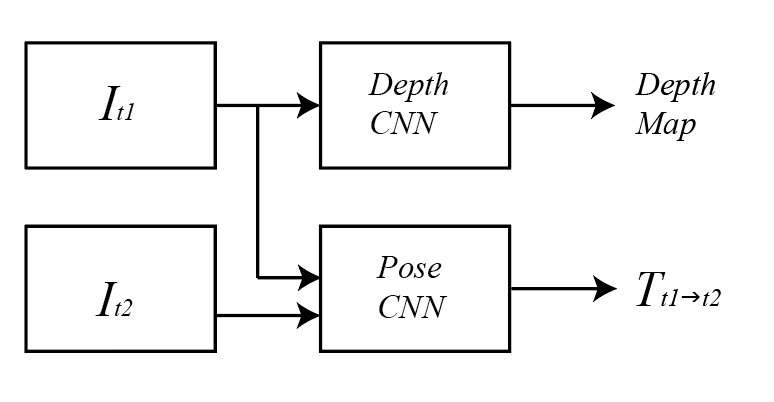
\includegraphics[width=3in]{images/cnns.png}
    \caption{Machine learning approaches have demonstrated strong results in simultaneously estimating depth maps and relative poses between images. Typically, a pair of CNN's is used, one for each task. The depth CNN is provided with the first view at $t=1$ and the pose CNN is provided both views.}
    \label{2cnns}
\end{figure}


While the training pipeline is unsupervised in the sense that labelled data is not required, some form of supervision signal is nevertheless required to optimise the parameters of the pair of networks. These papers take advantage of the fact that if the physical structure of a scene is known, then a novel rendering of that scene from a different viewpoint is achievable. Thus, \cite{garg2016unsupervised} suggested using photometric reconstruction as a supervision signal - from $I_{t2}$, reconstruct $I_{t1}$. The difference between the reconstruction and the real image can form a supervisory signal for the pair of networks. This work similarly uses photometric reconstruction as the principal supervisory signal in training a pair of networks to perform visual odometry and depth estimation. The photometric reconstruction loss is


\begin{equation}
    L_{photometric} = \sum_n^W \sum_m^H |I_{t1}(m,n) - \hat{I_{t1}}(m,n)|.
    \label{photometricloss}
\end{equation}


Humans can easily imagine what a scene will look like if we move our heads slightly, but only if we know the overall shape of the object we are looking at. Similarly, given two images separated by a small interval of time $I_{t1}$ and $I_{t2}$, one could synthesise what $I_{t1}$ would look like by sampling the pixels from $I_{t2}$, if the relative pose $T_{t1\rightarrow t2}$ between the two cameras and a pixel-wise depth of the scene $D_{t1}(p)$ is known. In practice, this can be done by obtaining the coordinates of the pixels in the first image $p_{t1}$ projected on to $I_{t2}$'s camera sensor. Assuming a pinhole model, the complete expression for $p_{t1}$'s projected location on the second camera, $\hat{p_{t2}}$ is 

\begin{equation}
\hat{p_{t2}} = KT_{t1\rightarrow t2} D(p_{t1}) K^{-1} p_{t1}.
\end{equation}

Here K represents the intrinsics matrix. In right-to-left order, this transform first maps each pixel to a ray direction using the inverse camera intrinsics $K^{-1}$. Each ray is then given a depth with the per-pixel depth map $D(p_{t1})$, producing a 3D point cloud. The transform $T_{t1 \rightarrow t2}$ transforms each point to the coordinate frame of the second camera, then the matrix $K$ projects each of those points onto the camera sensor of the second camera. The obtained coordinate $\hat{p_{t2}}$ is continuous, while pixel coordinates are discrete. A pixel value thus needs to be interpolated, keeping in mind that each step of a neural network pipeline must be differentiable to support the backpropagation of gradients. 

It was suggested by Zhou et al. \cite{zhou2017unsupervised} that adopting bilinear sampling could be used as a fully differentiable sampling mechanism. The use of bilinear interpolation as a differentiable sampling pipeline was first proposed Jaderberg et al. \cite{jaderberg2015spatialtransformer}, and adapted by Zhou et al. \cite{zhou2017unsupervised} to perform the differentiable image warp. A bilinear sampling kernel is described by 

\begin{equation}
    V = \sum_n^W \sum_m^H U_{nm} max (0, 1-|x - n|) max(0, 1-|y - m|).
\end{equation}

$V$ is the output of the sampling kernel, $U$ is the source image being sampled, $n$ and $m$ index over the columns and rows of the kernel respectively, $H$ and $W$ are the height and width of the sampling kernel, and $x$ and $y$ are the local coordinates of the sampling location. The $2 \times 2$ sampling kernel used to perform the photometric reconstruction is, in essence a weighted sum of the 4 nearest neighbour pixels, based on its proximity to those pixels. The equation is differentiable with respect to both x and y:


\begin{equation}
    \frac{\partial{V}}{\partial{x}} = \sum_n^W \sum_m^H U_{nm} max(0, 1-|y - m|).
\end{equation}
\begin{equation}
    \frac{\partial{V}}{\partial{y}} = \sum_n^W \sum_m^H U_{nm} max(0, 1-|x - n|).
\end{equation}

Using this bilinear sampling kernel, we can thus sample pixels from $I_{t2}$ to reconstruct $I_{t1}$ in a fully differentiable manner, allowing the backpropagation of gradients through the networks. The pipeline with photometric reconstruction as the supervision signal can be illustrated as shown in Figure \ref{supervisedMLCNNS}. Bilinear interpolation is similarly employed in this work to compute the photometric reconstruction loss of the estimated depth and pose. However, because this work operates on light fields, the output of photometric reconstruction won't be a single image, but a whole array of images.


\begin{figure}
    \centering 
    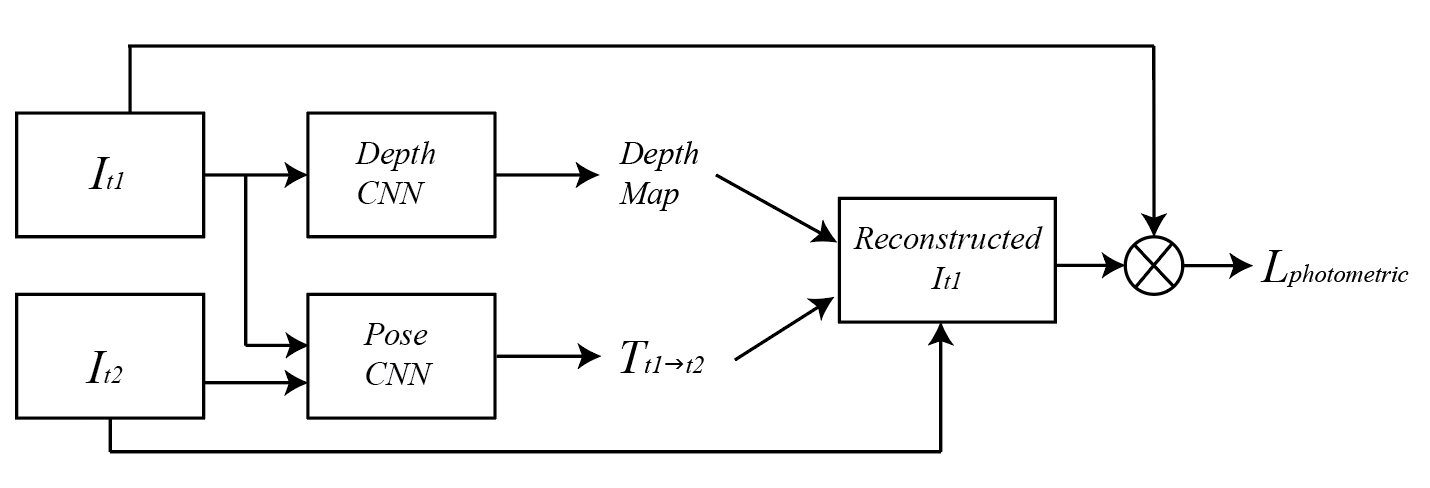
\includegraphics[width=5in]{images/mlpipeline.png}
    \caption{To provide a supervisory signal to the depth and pose CNN's, Garg et al. \cite{garg2016unsupervised} suggested using photometric reconstruction. The loss function is formulated by taking the difference between the reconstructed image $\hat{I_{t1}}$ and the actual image $I_{t1}$, shown in equation \ref{photometricloss}.}
    \label{supervisedMLCNNS}
\end{figure}


In addition to the photometric reconstruction loss providing the main supervision signal to the network, Zhou et al. \cite{zhou2017unsupervised} employs a smoothness loss to ensure that the produced depth map is globally smooth. The smoothness penalises the second order gradient of the image - i.e. the depth network is encouraged to produce a depth map characterised mostly by low-frequency components, and penalised for high-frequency components. Recognising that depth discontinuities frequently occur in parts of the image where a strong edge appears, Godard et al. \cite{godard2016consistency} on the other hand suggested the use of an edge-aware smoothness loss that also penalises large gradients in the depth map $\partial{d}$, but lowers the weight of the loss in regions where the image gradient $\partial{I}$ is large. 

\begin{equation}
    L_{smooth} =  \sum_n^W \sum_m^H |\partial_x d_{nm} e^{-|\delta_x I_{nm}|}| + \partial_y d_{nm} e^{-|\delta_y I_{nm}|}|
\end{equation}

There have been several iterations \cite{godard2016consistency, godard2018selfsupervised, zhan2018deepfeature} of this pipeline, most of which have focussed on introducing novel loss functions to improve the quality of the depth and pose estimates. To the best of our knowledge however, this pipeline has only ever been applied to monocular and stereo camera setups. While monocular and stereo cameras are ubiquitous in modern digital devices, this thesis will investigate the potential for the use of this pipeline to achieve improved results using a broader, more generalised family of imaging devices. 

Breaking free of the pinhole principle from which human eyes have developed and which commercial cameras have adopted, has wide implications in the field of machine vision. Reinforcing this idea is the rise in popularity of imaging techniques such as multi-spectral imaging, plenoptic cameras and polydioptric cameras, however interpreting ray directions and geometry for new cameras may not always be apparent, giving rise to the data-driven approach. Working on the principle that machine vision does not necessitate mimicking the human eye to capture imagery, this thesis investigates the capabilities of machine learning for querying depth and pose using one such novel imaging device - a camera array.



\section{Convolutional Neural Networks and Light Field Images}

In order to craft such a machine learning pipeline that complements the use of camera arrays, an investigation into input methods for 4D light fields into convolutional neural networks is due. It is recognised in Sun et al. \cite{sun2016lfdepthcnn} that while epipolar plane images (EPI) explicitly encode depth information, directly extracting such information without significant post-processing refinement and computational cost is difficult. The literature demonstrates strong results in using a CNN to interpret the gradient-depth relationship between an EPI and the images corresponding depth map. An EPI is extracted in both the horizontal and vertical direction for every row and column of the image in the $u, v$ plane, and subsequently fed to the network as two long, cubic volumes to obtain their results.

The rich textural data available in a 4D lightfield was purposed by Wang et al. \cite{wang2016lfcnn} for the task of material recognition using a deep CNN. In addition to reporting significantly improved material-recognition results (from 70\% to 77\% accuracy), \cite{wang2016lfcnn} proposes and compares a number of strategies for training on 4D images. One method that achieves strong results uses an angular filter, taking advantage of the 'angular resolution' that is gained by using a light field image over 2D images. The 4D light field image is first reshaped to form what is called a 'remap' image. To illustrate what a remap image looks like, a traditional 2D image is formed by discrete pixels, whereas a remapped 4D image on the other hand is formed of blocks of pixels, each block of size $h_a \times w_a$, formed by taking one pixel from each camera in the array. The result is a 2D image from which a 2D convolutional filter is able to learn features that indicate texture and parallax. While the remapping method achieved the best results, unfortunately such an arrangement of the image data does not make sense in the case of the camera array being used for this project as the cameras are arranged in a crosshair formation - 8 vertical cameras, 8 horizontal and 1 center image. The remapped image using this camera would comprise $17 \times 17$ blocks of mostly black pixels, producing a very inefficient representation of the data. 

Another method proposed in \cite{wang2016lfcnn}, albeit one that demonstrated lower accuracy than the angular filter method, was to concatenate images along their RGB channels prior to being fed to the network. The dimensionality of the image is quickly downsampled, and is thus a more computationally and memory efficient method than using angular filters, whilst still demonstrating improvement over 2D images. A potential improvement on this strategy that may prove useful in this work would be to use a dilated convolution, effectively opening the receptive field to a much larger area of the image without increasing computational complexity. Such a CNN would benefit from being able to sample a larger area of the image to recognise robust geometric features. 

These strategies each treat light field images as a volume of 2D images, and thus do not take full advantage of the 4D signal structures present in a light field. One possible improvement that might learn to more effectively utilise these 4D signals is to swap out the 2D convolutional filters typically used in image data for a 3D convolutional filter which is more commonly applied to video data. 
